% Informe técnico – Parte 5: Cartera de Inversión Pública (Datos Abiertos MEF)
% Compilar con: lualatex informe_parte5.tex
\documentclass[12pt,a4paper]{article}

\usepackage{fontspec}            % Latin Modern (igual al informe de módulos 3 y 4)
\usepackage{polyglossia}
\setdefaultlanguage{spanish}
\usepackage{amsmath,amssymb}
\usepackage{geometry}
\geometry{margin=2.8cm}
\usepackage{xcolor}
\usepackage{titlesec}
\usepackage{booktabs}
\usepackage{graphicx}
\usepackage{tabularx}
\usepackage{enumitem}
\usepackage{microtype}
\usepackage[hidelinks]{hyperref}
\usepackage{xurl}

\definecolor{azul}{RGB}{52,96,150}
\titleformat{\section}{\Large\bfseries\color{azul}}{\thesection}{1em}{}
\titleformat{\subsection}{\large\bfseries\color{azul}}{\thesubsection}{1em}{}
\setlist[itemize]{label=\textcolor{azul}{\scriptsize$\blacksquare$},leftmargin=1.4em,itemsep=2pt,topsep=4pt}
\setlist[enumerate]{leftmargin=1.6em,itemsep=3pt,topsep=4pt}
\newcolumntype{L}{>{\raggedright\arraybackslash}X}
\renewcommand{\arraystretch}{1.15}
\newcommand{\var}[1]{{\renewcommand{\_}{\textunderscore\allowbreak}\texttt{#1}}}
\setlength{\emergencystretch}{3em}

\begin{document}

\begin{center}
  {\Large\bfseries INFORME TÉCNICO: PROCESOS ETL Y\\[3pt] JUSTIFICACIÓN METODOLÓGICA\par}
  \vspace{6pt}
  {\large Módulo 5 (Cartera de Inversión Pública -- Datos Abiertos MEF)\par}
  \vspace{14pt}
  Departamento de Análisis: Piura \qquad --- \qquad Periodo: 2016--2021\par
  \vspace{10pt}
  16 de octubre de 2026
\end{center}
\vspace{10pt}

\section{Cartera de Inversión Pública (Datos Abiertos)}

\subsection{Selección de la fuente}

El portal de Datos Abiertos del MEF publica nueve conjuntos de datos en la categoría
\emph{Inversión Pública}. Se eligió \textbf{Detalle de inversiones} porque es el único que
contiene, a nivel de proyecto, todos los campos exigidos. Los demás se descartaron:
\emph{Estado situacional} está por producto y empieza en 2017; \emph{Formato 12B} solo
tiene la programación financiera por periodo; \emph{Cierre de inversiones} e
\emph{Inversiones desactivadas} son subconjuntos; \emph{Componentes}, \emph{Expedientes
técnicos}, \emph{Indicadores de brechas} y \emph{Directorio de operadores} no describen la
cartera de proyectos.

Las variables se identificaron con el \textbf{diccionario oficial}
(\var{Detalle\_Inversiones\_Diccionario.csv}, 68 variables) publicado junto al recurso:

\begin{center}\small
\begin{tabularx}{\linewidth}{@{}lll@{}}
\toprule
\textbf{Campo solicitado} & \textbf{Columna del MEF} & \textbf{Columna final}\\
\midrule
Código Único de Inversión & \var{CODIGO\_UNICO} & \var{cui}\\
Ejecutora & \var{NOMBRE\_UEI} & \var{ejecutora}\\
Nivel de gobierno & \var{NIVEL} (GN, GR, GL) & \var{nivel\_gobierno}\\
Sector & \var{SECTOR} & \var{sector}\\
Función & \var{FUNCION} & \var{funcion}\\
Costo del proyecto & \var{COSTO\_ACTUALIZADO} & \var{costo}\\
Grado de avance & \var{AVANCE\_FISICO} / \var{AVANCE\_EJECUCION} & \var{avance}\\
Fecha de inicio & \var{FEC\_INI\_EJECUCION} & \var{fecha\_inicio}\\
Fecha de fin & \var{FEC\_FIN\_EJECUCION} & \var{fecha\_fin}\\
Fecha de última ejecución & \var{ULTIMO\_DEVENGADO} & \var{fecha\_ult\_ejec}\\
\bottomrule
\end{tabularx}
\end{center}

\subsection{Estrategia y Justificación del Proceso de Extracción (Extract)}

Se usó la \textbf{descarga directa del CSV} desde el servidor de archivos del portal
(método 1 del cuaderno de la semana 5):

\begin{itemize}
  \item URL: \url{https://fs.datosabiertos.mef.gob.pe/datastorefiles/DETALLE_INVERSIONES.csv}
        (archivo nacional de 247 MB, actualizado el 13/10/2026).
  \item Departamento: \var{DEPARTAMENTO = "PIURA"}; verificación cruzada con
        \var{UBIGEO}, cuyos dos primeros dígitos deben ser \var{"20"}.
  \item Variables extraídas: los diez campos solicitados más \var{NOMBRE\_INVERSION},
        \var{ESTADO}, \var{SITUACION}, \var{UBIGEO} y las columnas de respaldo para montos
        (\var{MONTO\_VIABLE}, \var{DEVEN\_ACUMUL\_ANIO\_ANT}, \var{DEV\_ANIO\_ACTUAL}) y fechas
        (\var{FEC\_INI\_EJEC\_FISICA}, \var{FEC\_FIN\_EJEC\_FISICA}, \var{PRIMER\_DEVENGADO},
        \var{ULT\_FEC\_DECLA\_ESTIM}).
\end{itemize}

\textbf{Por qué la descarga directa y no la API ni el scraping.} El portal ofrece la API
\var{datastore\_search} (\var{resource\_id = f9cc4ba0-931a-4b70-86c9-eacbd8c68596}), pero
para este recurso devuelve \var{"records": null}, con o sin filtro por departamento. El
scraping estático con BeautifulSoup tampoco es viable: la página del dataset se genera con
JavaScript y \var{requests} no recibe los enlaces. La descarga directa es reproducible, no
depende de la estructura HTML y trae la versión más reciente cada vez que se ejecuta.

\textbf{Procedimiento.}
\begin{enumerate}
  \item \textbf{Descarga en memoria.} El CSV se lee desde un buffer (\var{BytesIO}), sin
        escribirlo en disco. Hasta tres intentos con 10 segundos de espera ante errores
        temporales (500, 503, conexión cortada); ante un 404 se detiene con un mensaje
        explícito, porque reintentar no lo resuelve.
  \item \textbf{Codificación.} Se detecta en los primeros 2 MB (UTF-8 con respaldo
        \emph{latin-1}); si el error de decodificación cae al final de la muestra, es solo
        un carácter acentuado cortado y el archivo se trata como UTF-8.
  \item \textbf{Control de columnas.} Antes de leer se verifica que las columnas
        esperadas existan en la cabecera; si el MEF cambia un nombre, se emite una
        advertencia.
  \item \textbf{Lectura por bloques.} Se lee en bloques de 50\,000 filas, solo con las
        columnas necesarias (\var{usecols}) y como texto (\var{dtype=str}); en cada bloque
        se conservan únicamente las filas de Piura. El departamento se compara tras
        estandarizar el texto (mayúsculas, sin tildes ni espacios extra).
  \item \textbf{Validación.} Si no se encuentra ninguna inversión de Piura, el proceso se
        detiene con error en lugar de continuar con una base vacía.
\end{enumerate}

\subsection{Decisiones de Transformación (Transform)}

\textbf{Estandarización.} Los nombres de columna se pasan a minúsculas. El CUI se convierte
a entero (\var{Int64}); se eliminan registros sin CUI y CUI duplicados (se conserva el
último). Las variables categóricas se normalizan (mayúsculas, sin tildes) para que, por
ejemplo, ``ADMINISTRACIÓN'' y ``ADMINISTRACION'' cuenten como la misma categoría. Los montos
se convierten a \var{float} retirando símbolos y separadores de miles.

\textbf{Fechas a \var{datetime}.} El archivo mezcla formatos, que se resuelven por patrón y
no por posición:

\begin{center}\small
\begin{tabularx}{\linewidth}{@{}lL@{}}
\toprule
\textbf{Formato en la fuente} & \textbf{Ejemplo y columnas}\\
\midrule
\var{aaaa-mm-dd hh:mm:ss} & \var{2018-05-01 00:00:00} (\var{FEC\_INI\_EJECUCION}, \var{FEC\_FIN\_EJECUCION})\\
\var{AAAAMM} (periodo SIAF) & \var{201806} (\var{PRIMER\_DEVENGADO}, \var{ULTIMO\_DEVENGADO}); se fija al día 1 del mes\\
\var{AAAAMMDD}, \var{dd/mm/aaaa} & Formatos de respaldo, por si cambian en futuras versiones\\
\bottomrule
\end{tabularx}
\end{center}

Las fechas fuera del rango 1990--2040 se consideran errores de registro y pasan a
\var{NaT}. Cada fecha usa una columna principal y, si está vacía, una de respaldo:
\begin{itemize}
  \item \var{fecha\_inicio}: \var{FEC\_INI\_EJECUCION} $\rightarrow$ \var{FEC\_INI\_EJEC\_FISICA} $\rightarrow$ \var{PRIMER\_DEVENGADO}
  \item \var{fecha\_fin}: \var{FEC\_FIN\_EJECUCION} $\rightarrow$ \var{FEC\_FIN\_EJEC\_FISICA}
  \item \var{fecha\_ult\_ejec}: \var{ULTIMO\_DEVENGADO} $\rightarrow$ \var{ULT\_FEC\_DECLA\_ESTIM}
\end{itemize}

\textbf{Grado de avance.} Ambos avances se llevan a escala 0--100. Para el proyecto $h$ se
prioriza el avance físico; si falta, el financiero, y si este también falta, se calcula con
el devengado acumulado:
\[
\text{avance}_h =
\begin{cases}
\var{AVANCE\_FISICO}_h & \text{si existe}\\[2pt]
\var{AVANCE\_EJECUCION}_h & \text{si no}\\[2pt]
100 \cdot \dfrac{\text{devengado\_acum}_h}{\text{costo}_h} & \text{si ninguno existe}
\end{cases}
\]
La columna \var{fuente\_avance} registra qué criterio se usó en cada proyecto
(\var{fisico}, \var{financiero}, \var{imputado\_cerrada}, \var{imputado\_sin\_ejecucion}),
con $\text{devengado\_acum}_h = \var{DEVEN\_ACUMUL\_ANIO\_ANT}_h + \var{DEV\_ANIO\_ACTUAL}_h$.

\textbf{Valores perdidos (NaN) y atípicos.}

\begin{center}\small
\begin{tabularx}{\linewidth}{@{}>{\raggedright\arraybackslash}p{0.42\linewidth}L@{}}
\toprule
\textbf{Condición} & \textbf{Tratamiento}\\
\midrule
Costo nulo o $\le 0$ & Se usa \var{MONTO\_VIABLE}; si tampoco es positivo, queda NaN y se excluye del ponderado\\
Avance físico nulo (1\,190 casos) & Se usa el avance financiero\\
Avance aún nulo, inversión cerrada & 100 \% (se completó la ejecución)\\
Avance aún nulo, sin devengado ni ejecución & 0 \% (no inició la ejecución)\\
Fecha de fin nula (324 casos) & Se usa la fecha de última ejecución; si tampoco existe y no está cerrada, se considera abierta hasta la fecha de corte\\
Fecha de inicio nula & Se usa el inicio físico (F12-B) o el primer devengado; si aún falta, la fecha de última ejecución\\
Ejecutora nula (21 casos) & Se conserva sin imputar; no afecta a los agregados\\
Avance $> 100$ \% (22 casos) & Se recorta a 100 y se marca en \var{avance\_excede\_100} (sobrecostos)\\
Fecha fuera de 1990--2040 & \var{NaT}\\
\bottomrule
\end{tabularx}
\end{center}

\textbf{Cartera 2016--2021 y proyecto activo.} Cada inversión tiene un periodo de ejecución
efectivo:
\[
\text{inicio}_h = \text{fecha\_inicio}_h, \qquad
\text{fin}_h = \max(\text{fecha\_fin}_h,\ \text{fecha\_ult\_ejec}_h).
\]
Un proyecto está \textbf{activo en el año} $t$ si su periodo se superpone con ese año:
$\text{inicio}_h \le 31/12/t$ y $\text{fin}_h \ge 01/01/t$. La cartera detallada conserva
las inversiones activas en al menos un año entre 2016 y 2021.

\textbf{Agregado anual departamental.} Con $A_t$ el conjunto de proyectos activos en el año
$t$, $c_h$ el costo y $a_h$ el avance:
\[
N_t = |A_t|, \qquad
\text{Costo}_t = \frac{1}{10^6}\sum_{h \in A_t} c_h, \qquad
\text{Avance ponderado}_t = \frac{\sum_{h \in A_t} c_h\, a_h}{\sum_{h \in A_t} c_h}
\]
El costo total se expresa en millones de soles. En el avance ponderado, un proyecto grande
pesa más que uno pequeño, de modo que refleja la proporción del monto de la cartera que se
ha ejecutado. Se verifica que el resultado esté entre 0 y 100.

\textbf{Formato long y ancho.} El agregado se construye en formato \textbf{ancho} (una fila
por departamento-año), que es la estructura que requiere el panel. Por consistencia con las
demás fuentes, se guarda además una versión \textbf{long} con \var{melt}: identificadores
\var{departamento} y \var{anio}, y columnas \var{indicador} y \var{valor}. La cartera
detallada se mantiene como base independiente; al panel (P06) solo se incorpora el
agregado anual.

\subsection{Carga y Resultados (Load)}

Las bases se guardaron en formato Parquet en la ruta relativa \var{output/} del módulo
(definida con \var{pathlib} a partir de la ubicación del script):
\begin{itemize}
  \item \var{inversion\_detalle.parquet}: cartera detallada, 2\,230 proyectos (CUI único).
  \item \var{inversion\_agregado.parquet}: agregado anual en formato ancho (6 filas).
  \item \var{inversion\_agregado\_long.parquet}: agregado en formato long (18 filas).
\end{itemize}

\begin{center}
\begin{tabular}{@{}lrrr@{}}
\toprule
\textbf{Año} & \textbf{Proyectos activos} & \textbf{Costo total (S/ mill.)} & \textbf{Avance ponderado (\%)}\\
\midrule
2016 & 344   & 4\,718.5  & 69.5\\
2017 & 403   & 6\,518.1  & 63.4\\
2018 & 651   & 9\,152.1  & 61.1\\
2019 & 987   & 15\,791.4 & 54.3\\
2020 & 1\,382 & 19\,939.6 & 58.2\\
2021 & 1\,793 & 26\,737.9 & 57.5\\
\bottomrule
\end{tabular}
\end{center}

De los 2\,230 proyectos, 1\,596 corresponden a gobiernos locales, 519 al gobierno nacional
y 115 al gobierno regional. Por función, Transporte concentra el mayor costo (S/ 11\,288
millones), seguido de Saneamiento (S/ 4\,982 millones) y Educación (S/ 4\,414 millones).
El avance de 1\,040 proyectos proviene del registro físico y el de 1\,190 del financiero.

\subsection{Resolución de problemas técnicos y limitaciones}

\begin{itemize}
  \item \textbf{API sin registros.} \var{datastore\_search} respondía con éxito pero sin
        datos; se optó por la descarga directa del CSV.
  \item \textbf{Servidor de archivos fuera de servicio.} El 15/10/2026 el servidor
        \var{fs.datosabiertos.mef.gob.pe} devolvía \emph{404 Not Found} para todos sus
        archivos, incluido el diccionario, aunque la página seguía mostrando el enlace. Se
        incorporaron reintentos y un mensaje de error explícito; el servicio se restableció
        el 16/10/2026 y el proceso se ejecutó sin modificar el código.
  \item \textbf{Archivo pesado.} Los 247 MB nacionales se procesan por bloques y solo con
        las columnas necesarias, para no saturar la memoria.
  \item \textbf{Solo inversiones activas.} Todos los registros del archivo tienen
        \var{ESTADO = ACTIVO}; las inversiones cerradas se publican en otro conjunto
        (\emph{Cierre de inversiones}). Por ello la cartera de los primeros años está
        \textbf{subestimada}: faltan los proyectos que se ejecutaron entonces y ya se
        cerraron. Esto explica en parte el crecimiento de 344 a 1\,793 proyectos.
  \item \textbf{Avance a la fecha de corte.} El avance corresponde a la última
        actualización del archivo (octubre de 2026), no al cierre de cada año. El avance
        ponderado anual mide, por tanto, cuánto se ha ejecutado \emph{hoy} de la cartera
        que estaba activa en cada año.
\end{itemize}

\section*{Anexo obligatorio: Registro de consultas (prompts a IA)}

Se detalla la bitácora de interacción utilizada durante el desarrollo del módulo 5:

\begin{enumerate}[label={[\arabic*]},leftmargin=2.2em,itemsep=4pt]
\item ¿Por qué me genera este error?\\[4pt]
      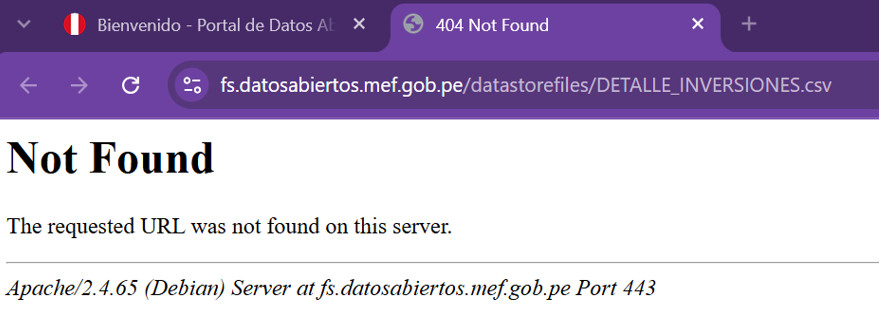
\includegraphics[width=0.85\linewidth]{error404.png}
\item ¿Qué es CKAN?
\item Voy a seleccionar Detalle de inversiones, pero ¿puedo escoger otros datasets que encajan con cartera de inversiones, como el de Estado situacional de inversiones?
\item ¿Es debido al navegador que se genera ese error 404?
\item Con esa previsualización de etiquetas, crea una lista de columnas.
\item Ayúdame a mejorar este código para descargar el CSV completo.
\item Explícame estas librerías: \var{logging} y \var{unicodedata}.
\item ¿Para qué sirve uncode y decode?
\item No funciona el código que hice. ¿Crees que se deba al error 404 de la página donde se obtienen los datos? ¿Cuánto tiempo tengo que esperar?
\item En la parte de Transform, ¿me dice que pase de long a ancho en la evaluación?
\item El que me diste.
\item El que me diste.
\item Explícame qué es un archivo Parquet.
\item ¿Cómo generar como resultado un archivo Parquet?
\item Dime cómo podría crear un informe técnico. ¿Sería explicando cada archivo .py de extract, transform y load?
\end{enumerate}

\end{document}
